% Options here are passed to the article class.
% Most common options: 10pt, 11pt, 12pt
\documentclass[10pt]{datasheet}

% Input encoding and typographical rules for English language
\usepackage[utf8]{inputenc}
\usepackage[english]{babel}
\usepackage[english]{isodate}

% tikz is used to draw images in this example, but you can
% also use \includegraphics{}.
\usepackage{graphicx}

% These define global texts that are used in headers and titles.
\title{CH01: Parallelized Encoded Chest Hall}
\author{Andrews54757}
\tags{chest-halls, parallelized, decimal-encoding, hopperlocked, 10-chests}
\date{October 2022}
\revision{Revision 1}

\begin{document}
\maketitle

\section{Features}

\begin{itemize}
\item{800 chests, 10 chests per slice with 24 blocks of width}
\item{Fully parallelizable (19x hopperspeed for items, 1x hopperspeed for box insertion)}
\item{100\% hopperlocked with sectional unlocking}
\item{10/8 gt streamed comparator outputs}
\item{Self-repairable toggle states with Auto-Fix sequence}
\item{Low active lag, +1 ms at 1x HS, +6 ms at 20x HS}
\end{itemize}

\section{General Description}
The CH01 is a fully hopperlocked 10 item per slice encoded chest hall with a backend sporting up to 20x HS parallelization. It is able to insert both loose items and boxes into chests allowing for item/box hybrid functionality.

The transport mechanism for this hall does not support overflow protection. Extra items may despawn. It is recommended that the comparator readouts are used to limit the insertion amounts as needed to prevent overflow.

Comparator readouts are streamed from the chests at 10 codes / 8 gt. This is initiated by a pulsed signal.

All toggle states are self-repairable. The repair process is initiated by a pulsed signal.
% Switch to next column
\vfill\break

\begin{figure}[h]
    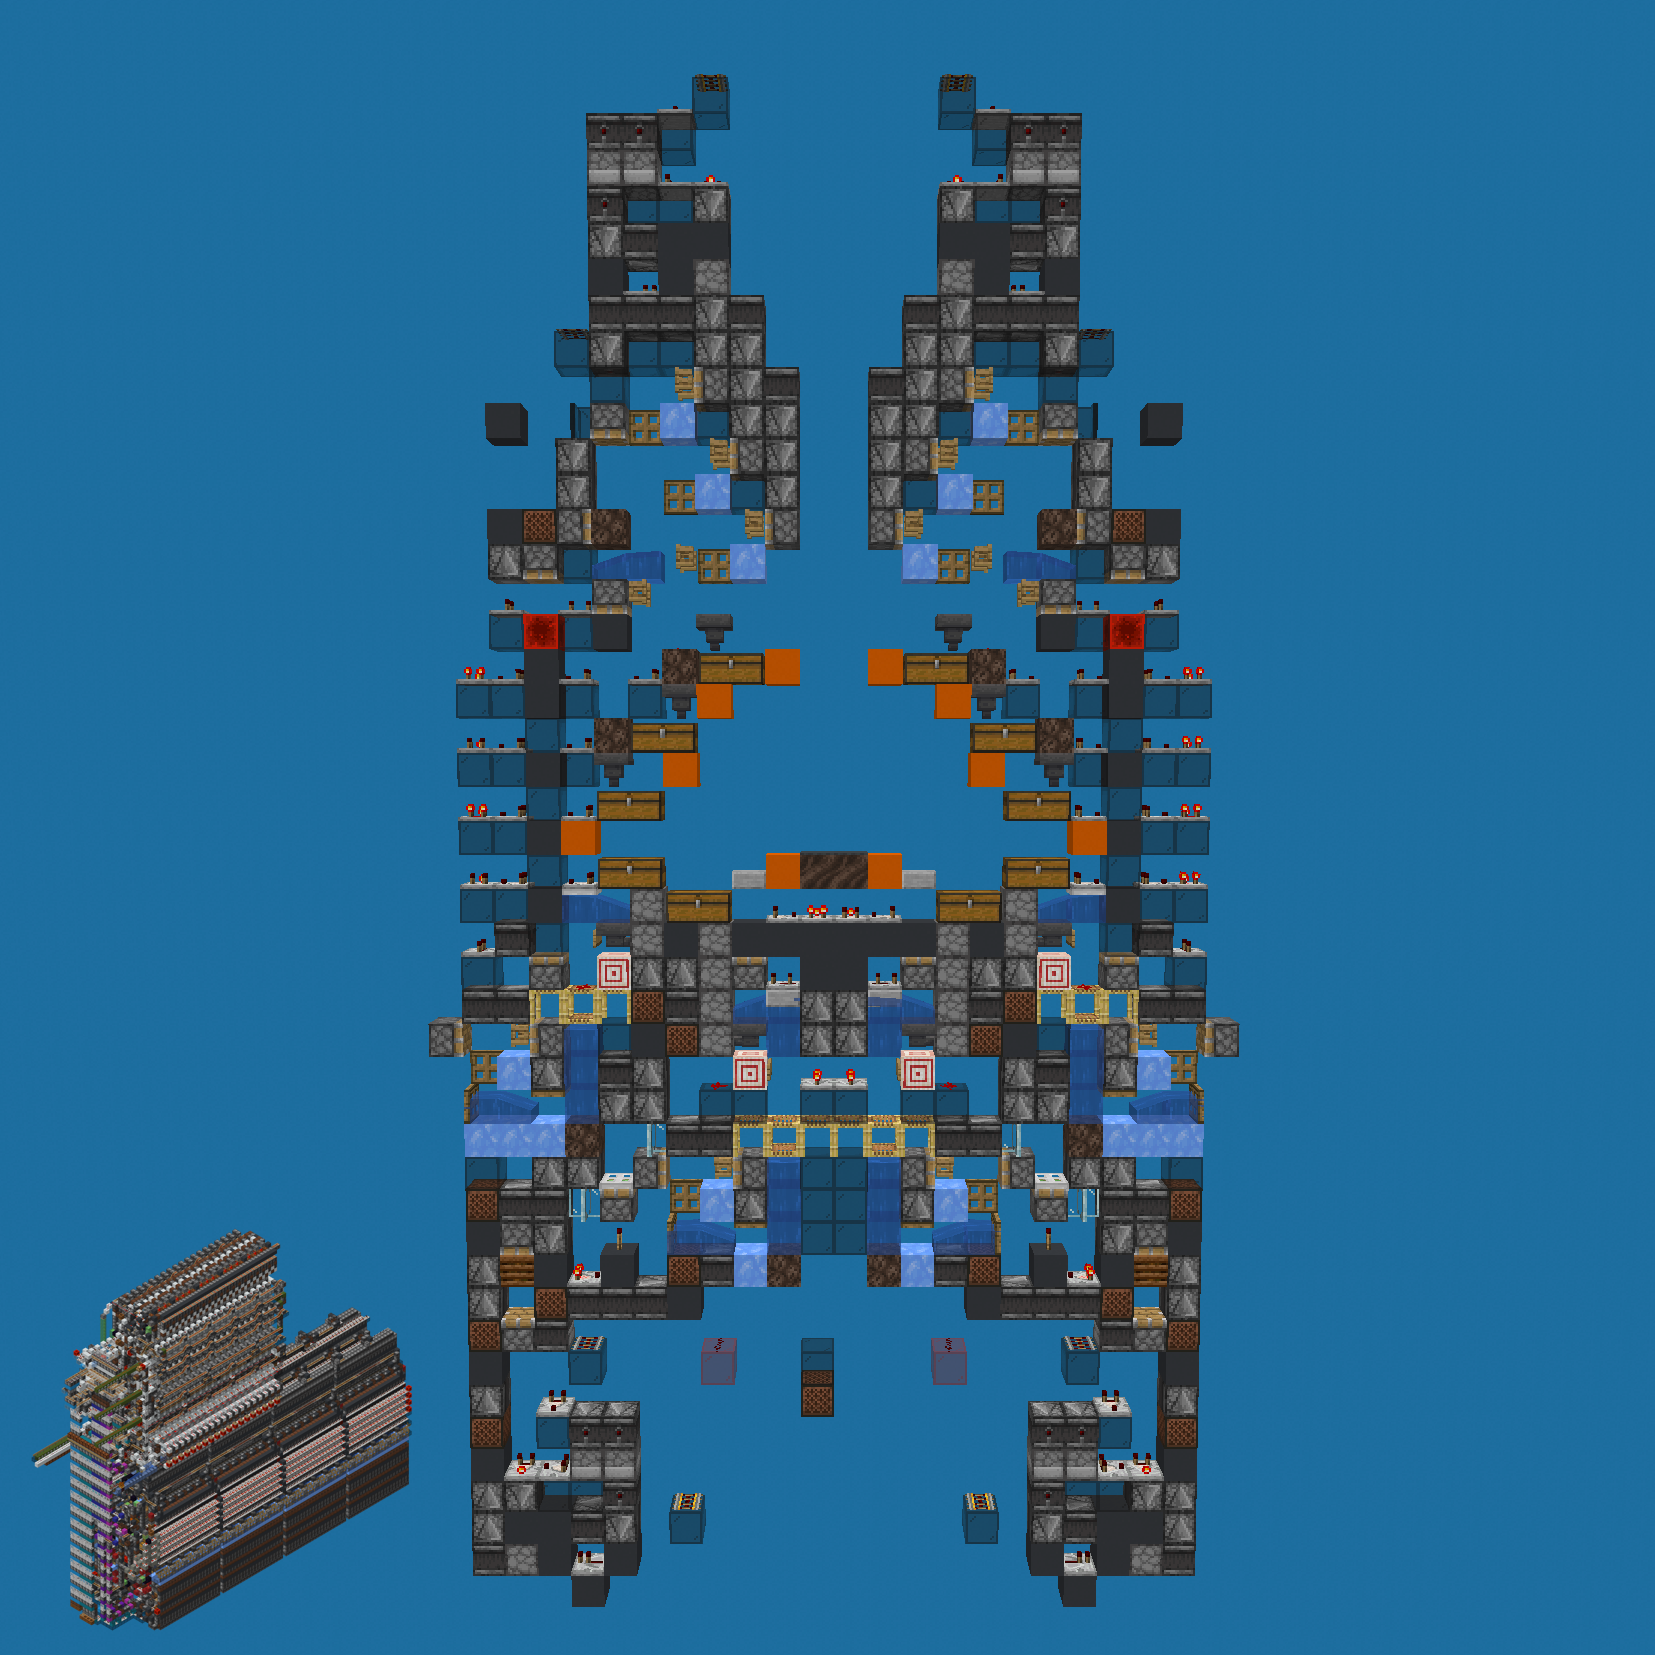
\includegraphics[width=0.45\textwidth]{chesthall.png}
    \caption{Chest Hall Slice}
\end{figure}

% For wide tables, a single column layout is better. It can be switched
% page-by-page.
\onecolumn
\section{Device Specifications}

\begin{table}[h]
    \caption{Inputs}
    \begin{tabularx}{\textwidth}{l | c | X}
        \thickhline
        \textbf{Name} & \textbf{Range} & \textbf{Description} \\
        \hline
        Item Code 1 & 1-10 & First digit indicating chest location in slice. \\
        Item Code 2 & 1-8 & Second digit indicating horizontal section. \\
        Item Code 3 & 1-10 & Third digit indicating slice location in horizontal section. \\
        \hline
        Max Slot Count & 1-14 & Maximum number of slots to fill given by $value*4$\\
        \hline
        Is Unstackable & 0-1 & Indicates item type is unstackable.\\
        Is 16-Stackable & 0-1 & Indicates item type is 16-stackable.\\
        Is 64-Stackable & 0-1 & Indicates item type is 64-stackable.\\
        \hline
        Box Mode & 0-1 & Indicates that box items should be inserted directly without unloading\\
        \hline
        Append Mode & 0-1 & When true, boxes will be added to slices already unloading the item type instead of rejecting the order. WARNING: Can break unloaders with certain timings when TRUE. \\
        \hline
        Execute Order & Pulse & Executes the order with the given settings. \\
        Read Comparators & Pulse & Reads and streams comparator readings. \\
        Auto-Fix & Pulse & Initiates auto-fix sequence \\
        \hline
        Item Input & Item & Box item to be inserted/unloaded. \\
        \thickhline
\end{tabularx}
\end{table}

\begin{table}[h]
    \caption{Outputs}
    \begin{tabularx}{\textwidth}{l | c | X}
        \thickhline
        \textbf{Name} & \textbf{Range} & \textbf{Description} \\
        \hline
        Item Code 1 & 1-10 & First digit indicating chest location in slice. \\
        Item Code 2 & 1-8 & Second digit indicating horizontal section. \\
        Item Code 3 & 1-10 & Third digit indicating slice location in horizontal section. \\
        \hline
        Remaining Slot Count & 1-14 & Remaining number of slots to fill given by $value*4$\\
        \hline
        Ready & 0-1 & Indicates that the system is ready to execute the next order.\\
        \hline
        Unfulfilled & Pulse & Indicates that desired slot count was greater than what could be inserted. Followed by item code and remaining slot count signals. \\
        \hline
        Item Output & Item & Output for empty boxes and rejected query boxes. \\
        \thickhline
\end{tabularx}
\end{table}
\newpage
\section{Device Specifications Contd.}
\begin{table}[h]
    \caption{Device Specifications}
    \begin{tabularx}{\textwidth}{l | c c c | c | X}
        \thickhline
        \textbf{Parameter} & \textbf{Min.} & \textbf{Typ.} & \textbf{Max.} &
        \textbf{Unit} & \textbf{Conditions} \\
        \hline
        Input Throughput  & - & - & 1 & HS & \multirow{2}{*}{Normal Usage} \\
        Output Throughput  & 1 & - & 20 & HS & \\
        \hline
        Order Execution Interval & 88 & 106 & - & gt & Dependant on unloader's used capacity\\
        \hline
        Passive Lag & 1.5 & 2.8 & 3.5 & ms & \multirow{2}{6cm}{Ryzen 5 3600, 2GB RAM. MC 1.18.1 with Lithium.} \\
        Active Lag & +1 & - & +6 & ms & \\
        \hline
        Hopper Count & & 884 & & Hoppers & \\
        \hline
        MC Version & 1.16 & 1.18.2 & - & MCV & Latest version at time of writing: 1.19.2\\
        \hline
        Dimensions & & 24 x 91 x 108 & & Blocks & \\
        \thickhline
\end{tabularx}
\end{table}

\section{Testing Data}

\begin{table}[h]
\caption{Executed Tests}
\begin{tabularx}{\textwidth}{l | X}
    \thickhline
    \textbf{Test} & \textbf{Result} \\
    \hline
    Item Stackability and Max Slots & Unstackable, 16 stackable, and 64 stackable items were successfully input into the system with varying maxinum slot counts without overflowing.\\
    \hline
    All Chests & Two boxes of items were successfully unloaded and inserted into every chest with no loss.\\
    \hline
    Box Mode & Boxes were successfully inserted into multiple chests with no loss.\\
    \hline
    Unloader Component & Hundreds of thousands of items were passed through unloader modules without loss. All empty boxes were collected. Varying box fill levels and premature abort was tested successfully.\\
    \hline
    Auto-Fix Toggles & The storage was purposefully broken at various toggles and a repair was attempted with the auto-fix sequence. The system was always successfully repaired with multiple invokations of the auto-fix sequence.\\
    \thickhline
\end{tabularx}
\end{table}

\section{Download Information}
\begin{table}[h]
    \caption{Download Information}
    \begin{tabularx}{\textwidth}{l | l | l | X}
        \thickhline
        \textbf{Identifier} & \textbf{MC} & \textbf{File} & \textbf{Description} \\
        \hline
        CH01 & 1.18.2 & \href{https://github.com/Soontech-Annals/Archive/blob/92d3541e07ddc3ab90360e923907f040eca76834/Archive/chest-halls/CH01\%20Parallelized\%20Encoded\%20Chest\%20Hall/CH01\_encoded\_chest\_hall\_p30.litematic?raw=1}{CH01\_encoded\_chest\_hall\_p30.litematic} & Litematic of chest hall with inventories. \\
        \thickhline
    \end{tabularx}
\end{table}

\newpage
\section{Related Components}
\begin{table}[h]
    \caption{Related Components}
    \begin{tabularx}{\textwidth}{ l | l }
        \thickhline
        \textbf{Identifier} & \textbf{Description} \\
        \hline
        DC02 & 10BPS 2 Digit Decimal Decoder \\
        \thickhline
    \end{tabularx}
\end{table}
\end{document}


